\documentclass{article}%
\usepackage[T1]{fontenc}%
\usepackage[utf8]{inputenc}%
\usepackage{lmodern}%
\usepackage{textcomp}%
\usepackage{lastpage}%
\usepackage[head=40pt,margin=0.5in,bottom=0.6in]{geometry}%
\usepackage{graphicx}%
%
\title{\textbf{Dialogar hasta la extenuación}}%
\author{RAFAEL DEL NARANCO}%
\date{04/03/2019}%
%
\begin{document}%
\normalsize%
\maketitle%
\textbf{URL: }%
http://www.eluniversal.com/el{-}universal/34506/dialogar{-}hasta{-}la{-}extenuacion\newline%
%
\textbf{Periodico: }%
EU, %
ID: %
34506, %
Seccion: %
el{-}universal\newline%
%
\textbf{Palabras Claves: }%
NO\_TIENE\newline%
%
\textbf{Derecho: }%
2.1%
, Otros Derechos: %
\newline%
%
\textbf{\textit{No podemos seguir agraviándonos con injurias, y aunque las posiciones ideológicas puedan estar separadas, siempre será más valioso lo que nos une como patria. Conversa hasta llegar a un acuerdo...}}%
\newline%
\newline%
%
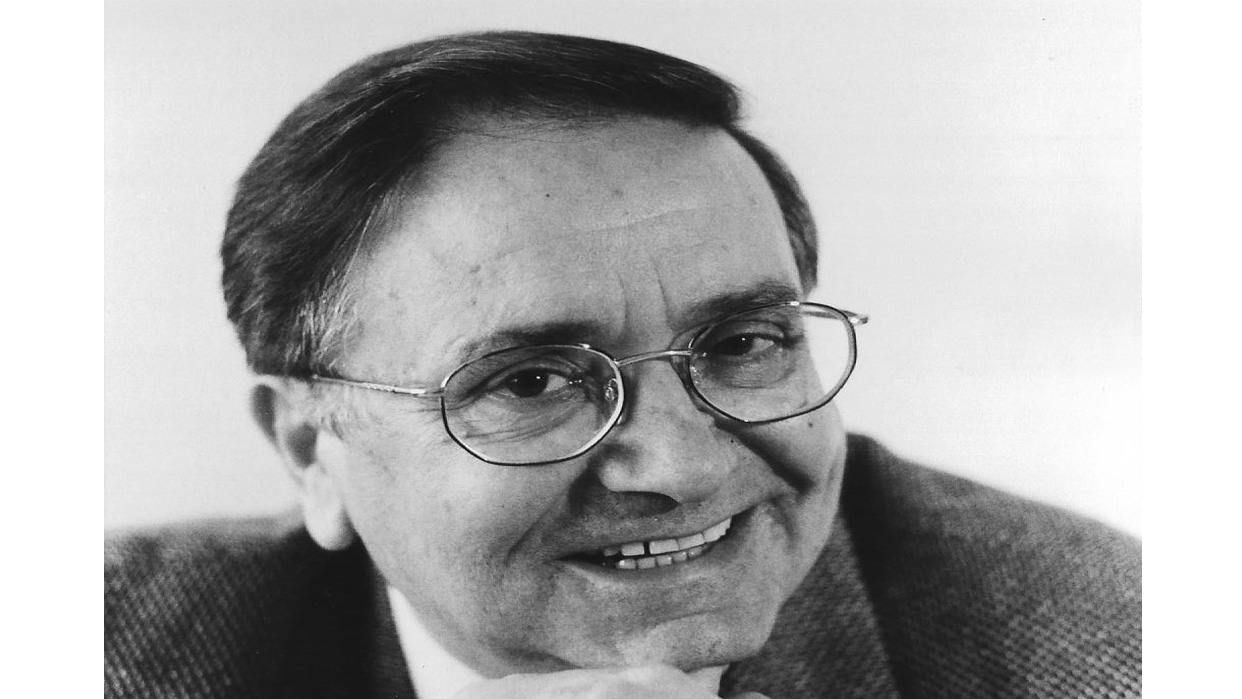
\includegraphics[width=300px]{EU_34506.jpg}%
\newline%
%
Las ideologías más sacudidas en el planeta {-}liberalismo, socialismo, radicalismo, fascismo, comunismo y monarquía en todos sus estamentos{-}, son elementos sociales de la raza humana que han estado, de una forma u otra, unidos al destino de cada uno de nosotros. No lo olvidemos: nadie es una isla, y cuando se trata de política somos la arenilla con la que se construye una sociedad.%
\newline%
%
Lo dicho no es una entelequia, es la expresión de como nos gobiernan. Por supuesto, no estamos creando un concepto político ni recreándonos en sus avatares, simplemente percibimos sus derivaciones.%
\newline%
%
Decir que vamos en la Venezuela actual de mal en peor, es reflejar una realidad de miedos y desasosiego que nos sofoca. El país se halla envuelto en una sinrazón con un gobierno uncido a una tabla de salvación que cree legalista y que hace agua a borbotones.%
\newline%
%
Es bien que los pueblos de la noche a la mañana no se hunden ni desaparecen: imperecederamente se levantan de sus propias cenizas, aunque suelen quedar maltrechos con profundas angustias en sus entrañas, y en esa marabunta acongojante nos hallamos ahora mismo.%
\newline%
%
El panorama es desolador, con un gobierno navegando entre piélagos de niebla mantenido con correas milicianas.%
\newline%
%
La negrura es plena. No parece que nos entendamos. Hay dos países y a uno de ellos, el chavismo, tras 20 años de gobierno, le falla el norte de la prudencia política. Si se retira ahora por propia voluntad ante las grandes grietas que presenta, puede, en la oposición, hacer examen de conciencia, analizar errores, y organizarse. No siempre el poder está en los aposentos gubernamentales.%
\newline%
%
Conversemos para entendernos y crear puentes de convivencia. Le decimos a Nicolás Maduro: “Un mal político piensa nada más que en las elecciones. Un estadista en la próxima generación”.%
\newline%
%
Hermandad%
\newline%
%
Hace un tiempo no tan lejano teníamos un territorio en el que, a pesar de sus deslices, aún se podía vivir, había libertad y los venezolanos poseían un sentido de hermandad. La patria no se hallaba tan profundamente dividida como lo está hoy y los presidentes ni soñaban con perpetuarse en el poder en nombre de una rebelión quimérica, personalista y decante.%
\newline%
%
Nunca he creído en estas revoluciones, sino en los cambios paulatinos de las sociedades bajo el predominio de valores intrínsecos e inviolables.%
\newline%
%
Y añadamos lo que decía Günter Grass: “Me asustan sus aspiraciones absolutas, su intolerancia”… Las revoluciones han sustituido dependencia por dependencia y un yugo por otro yugo”.%
\newline%
%
Venezuela, como oficio o marabunta de desatinos, parece una entelequia, una de esas irrealidades que nos apabullan, desganan y hacen posible un desasosiego general en medio de una apatía sempiterna.%
\newline%
%
El gobierno chavista es una idea inconclusa, mientras la oposición, que iba dando tumbos, se ha organizado y ha encontrado a un joven político, Juan Guaidó, con carisma, coraje y esa fuerza natural de los que tienen voluntad, anhelos limpios, y lo más importante en política, un liderazgo natural, consistencia, ética y una juventud que por sí misma no se halla aún contaminada de la rancia política.%
\newline%
%
Ahora mismo ya no somos una nación en su concepto más amplio. Nos hemos convertido en la visión quijotesca de un solo hombre, y hay sobre el ánimo general un desasosiego insondable, mientras la economía, como tal, ya no existe. Venezuela está hendida funestamente.%
\newline%
%
Dialogar sin descanso%
\newline%
%
Dialogar perennemente, sin descanso. Conversar por encima de las tumbas con el otro que, si se reflejara en un espejo sinuoso, terminaría representando la imagen de nuestra propia apariencia.%
\newline%
%
No podemos seguir agraviándonos con injurias, y aunque las posiciones ideológicas puedan estar separadas, siempre será más valioso lo que nos une como patria.%
\newline%
%
Sin darnos cuenta, todos somos un poco descendientes de la esencia helénica y amamantamos la aventura del pensamiento. Allí nació una de las cualidades que hizo al hombre universal: el diálogo. Es decir, el pensamiento compartido en las conversas que iniciara Platón y continuara Aristóteles.%
\newline%
%
Y recordemos el valor de la libertad que algunas veces se nos olvida al estar trajinado el pan muestro de cada día, tan difícil de conseguir en estos tiempos. “La libertad es para el cuerpo social lo que la salud para cada individuo. Si el hombre pierde la salud ya no disfruta de placer alguno en el mundo; si la sociedad pierde la libertad, marchitase y llega a desconocer sus genes”.%
\newline%
%
En la mitad del medio, cuando el país dejó de ser gris para volverse bruno, había llegado el momento de regresar con ahínco al título de esta columna: dialogar, conversa sin descanso con el único fin de llegar a ese acuerdo que permita el resurgir de un nuevo consenso de todos, con ideas dignas, gente nueva y esperanzas frescas.%
\newline%
%
rnaranco@hotmail.com%
\newline%
%
\end{document}